% We use report since it is similar to book just doesn't use a blank page after every chapter
\documentclass[a4paper, 11pt]{report}
\usepackage{color}
\usepackage[english]{babel}
\usepackage{fullpage}
%Andrey required packages
\usepackage[table]{xcolor}
\usepackage{listings}
% For adding graphics/figures
\usepackage{graphicx}
\graphicspath{ {images/} }
% To make sure a figure is put where you specify use [H] option
\usepackage{float}
% The caption size
% http://tex.stackexchange.com/questions/101591/setting-font-size-for-caption-package
\usepackage[skip=2pt, font=small, labelfont={sf,bf}, margin=1cm]{caption}
% To get nice urls
\usepackage{url}

\begin{document}

% Add separate titlepage
\begin{titlepage}
    \begin{center}
        \vspace*{4cm}
        
        \LARGE
        \textbf{\LaTeX{} group assignment}
        
        \vspace{0.5cm}
        \large
        Using \LaTeX{} and VCS
        
        \vspace{1.5cm}
        
	\textbf{Andrey Afanas'yev}
	\\
	\textbf{Hamza Boulakhrif}
	\\
	 \textbf{Jorian van Oostenbrugge}
	
	\vspace{4.5cm}
	
	\begin{figure}[H]
    		\centering
    		
\includegraphics[scale=0.1]{uva}
	\end{figure}
        
        \vfill
        
        \vspace{0.8cm}
	SNE 2014
	\\
        \today
        
    \end{center}
\end{titlepage}


% remove all numbering but still add to ToC
\setcounter{secnumdepth}{-2}
\tableofcontents

% All content i.e. create a separate page in the chapters folder to include here
% use \chapter{<chapter name>} to add a title, use \input{chapters/<chapter name>}
\chapter{Week 36}
% This file contains all homework from week 36
% use \section{<name>}  to create a section per homework assignment
%Andrey required packages
%\usepackage[table]{xcolor}
%\usepackage{listings}

\section[Homework 1.2]{Homework 1.2: AJAX and XML}

\subsection{History}
In early 90’s of XX century most of websites were just a plain html pages. To access recent information from the page user are required to refresh page manually. This was an inefficient method of representing information on the web. Moreover, it leads to an additional load on the server and expands the bandwidth.
\begin{itemize}
\item In 1996, Microsoft presented the first basic solution for this problem. An iframe tag was implemented in to Microsoft Internet Explorer. The iframe tag allows splitting page in to segments. Each segment contains another HTML document. The iframe standardized in HTML 4.0 Transitional and could be used in HTML5.
\item However, the iframe does not solve the problem. In 1998, the Microsoft tem firstly implemented in Outlook Web App the XMLHTTP component that client can execute by a script. 
\item In 1999, Microsoft updated the iframe technology with an XMLHTTP ActiveX object that was introduced in Internet Explorer 5. Mozilla, Safari, Opera and other browser later adopted this technology as the XMLHttpRequest JavaScript object. Later multiple web applications began to use this technology like Outlook Web App (2000), Oddpost (2002) and Gmail (2004).
\\
\item AJAX World Wide Web Consortium on 5 April 2006 published the first specification draft XMLHttpRequest object as an attempt to create an official Web standard\cite {wk01}.
\end{itemize}


\subsection{Technology}
According Jesse James Garrett, the announcer (18 February 2005) of the term Ajax (short for asynchronous JavaScript + XML):
\begin{quote}
Ajax isn’t a technology. It’s really several technologies, each flourishing in its own right, coming together in powerful new ways.\cite {jj05}
\end{quote}
Indeed Ajax consist out of the following technologies:
\begin{center}
    \begin{tabular}{l|l p{7cm}}
    \rowcolor{cyan}
    \textbf{Technology} & \textbf{Role} \\ \hline
    \rowcolor{cyan!50}
    (X)HTML and & CSS Content presentation. \\ 
    \rowcolor{cyan!10}
    DOM	& Data display and interaction. \\ 
    \rowcolor{cyan!50}
    XML	& Data interchange. \\ 
    \rowcolor{cyan!10}
    XSLT & Data manipulation. \\ 
    \rowcolor{cyan!50}
    XMLHttpRequest & Asynchronous communication. \\
    \rowcolor{cyan!10}
    JavaScript & Brings al technologies together. \\ 
    \end{tabular}
\end{center}

\subsection{Workflow}
Figure~\ref{fig:ajax} shows ajax work flow sequence\footnote{Founded on http://www.w3schools.com/ajax/ajax\_intro.asp at 10-09-2014.}: 
\begin{center}
	\begin{figure}[h!]
	  \centering
		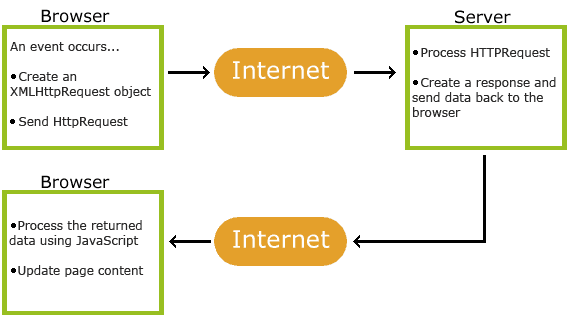
\includegraphics[scale=0.8]{ajax}
	  \caption{Ajax workflow}
	  \label{fig:ajax}
	\end{figure}
\end{center}

\newpage

\subsection{Example}
Below is an example, the comments should gave a clear picture of technologies interaction\cite{w3s}.
\lstset { %
    language=HTML,
    backgroundcolor=\color{black!5}, % set backgroundcolor
    basicstyle=\footnotesize,% basic font setting
}

\begin{lstlisting}
<! --standard  html file configuration-->
<!DOCTYPE html>
<html>
<head>
<!--Javascript-->
<script> 
function loadXMLDoc()
{
var xmlhttp;
//Definition of XMLHttpRequest object
if (window.XMLHttpRequest)
  {// code for IE7+, Firefox, Chrome, Opera, Safari
  xmlhttp=new XMLHttpRequest();
  }
else
  {// code for IE6, IE5
  xmlhttp=new ActiveXObject("Microsoft.XMLHTTP");
  }
xmlhttp.onreadystatechange=function()
  {
  if (xmlhttp.readyState==4 && xmlhttp.status==200)
    {
//Interaction with a html
    document.getElementById("myDiv").innerHTML=xmlhttp.responseText;
    }
  }
// Loading data defined in a xml file.
xmlhttp.open("GET","data.xml",true);
xmlhttp.send();
}
</script>
<!—continuing with a html -->
</head>
<body>
<h2>Unchangeable Text</h2> 
<div id="myDiv"><h2>Let AJAX change this text</h2></div>
<button type="button" onclick="loadXMLDoc()">Change Content</button>

</body>
</html>
</code>

\end{lstlisting}
\subsection{Conclusion}
Due some difficulties with AJAX and a required asynchronous data request AJAX slightly will be replaced by a JSON.
The JSON (JavaScript Object Notation), is an open standard format(RFC 7159) that uses human-readable text to transmit data objects. It is an alternative to XML and AJAX. Therefore, JSON is often used instead (see AJAJ), and the requests do not need to be asynchronous.\cite {wk02}

\chapter{Week 37}
% This file contains all homework from week 37
% use \section{<name>}  to create a section per homework assignment

\section[Homework 2]{Homework 2: Recursive Make Considered Harmlful}

In this section we'll describe the solutions for the "Recursive Make" problem as originally described in \cite{make_harmful}.
The three main solutions are explained in detail below:
\begin{description}
	  \item[Reshuffle] \hfill \\
	  Manually tweak the order of the modules in the top-level \textit{Makefile}. This is necessary because \textit{make} uses the postorder transversal, see figure \ref{fig:postorder}, but when dividing the DAG into two pieces, \textit{make} is not allowed to do so. The project dictates the order of transversal, but the order is plain wrong.  \hfill \\
	\begin{figure}[H]
		\centering
		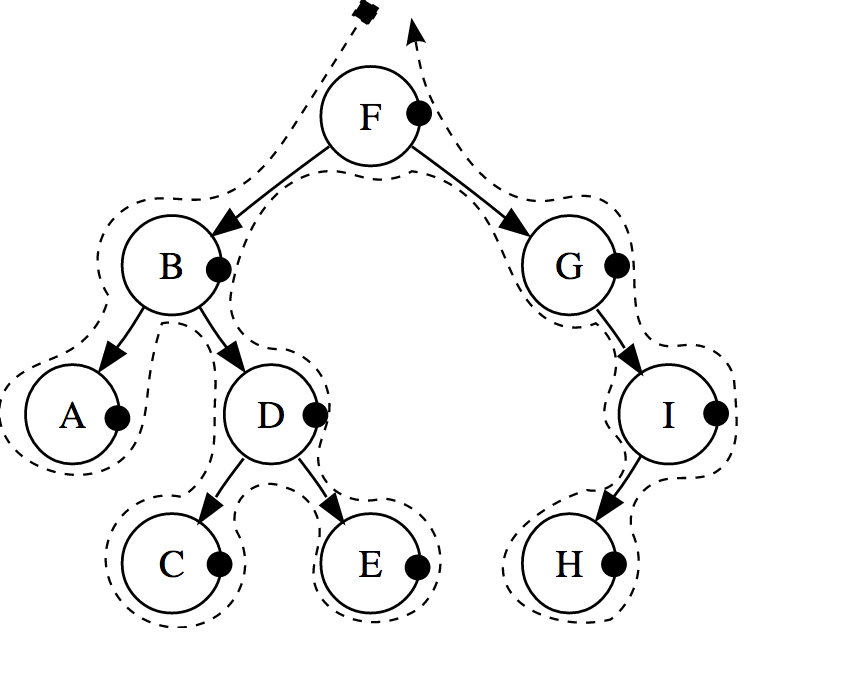
\includegraphics[scale=0.5]{postorder}
		\caption{The postorder traversal the sequence is: A, C, E, D, B, H, I, G, F \cite{postorder}}
		\label{fig:postorder}
	\end{figure}
	  \item[Repetition] \hfill \\
	  This solution tells \textit{make} to make more than one pass in the top-level \textit{Makefile}, an example is shown in script \ref{make_code} \hfill \\
	\begin{lstlisting}[frame=single, language=make, caption={An example Makefile using repetition.}, label={make_code}]
	 MODULES = ant bee 
 	all:
    	for dir in $(MODULES); do \
      		(cd $$dir; $(MAKE) all;) \
    	done
    	for dir in $(MODULES); do \
      		(cd $$dir; $(MAKE) all;) \
    	done 
	\end{lstlisting}
	This will double the time it takes to preform the build. But worse, the upper bound for the number of passes is proportional to the number of graph edges which are linked to multiple modules.
	
	  \item[Overkill] \hfill \\
	As the name suggests, this is like doing to much work. You could threat every dependency as always out of date and thus always - even if nothing changed - rebuilt files with dependencies. This solution will fail in non-deterministic ways when make uses the parallel build option (-j).  
	\end{description}
\chapter{Week 38}
% This file contains all homework from week 38
% use \section{<name>}  to create a section per homework assignment

\section[Homework 4]{Homework 4: XUTools}

XUTools manipulate files in terms of language-specific constucts, like C functions, IOS interface blocks and XML elements.


Traditional Unix Tools work on regular languages which don't work well with hierachical object models. Therefore the goal is to extend unix tools and the kind of languages they work on from regular languages to context-free languages.


XUTools presents eXtended Unix text-processing tool (XUTools) that enable extracting, counting and comparing in terms of language-specific constructs. The XUTools use a library of language grammars and xupath which is an xpath-like querying language to perform its operations. The following tools are considered the XUTools:

\begin{itemize}
	\item \textit{xugrep}
	\item \textit{xuwc}
	\item \textit{xudiff}
\end{itemize}

The goal is to extend more traditional unix tool into their extended form.

The eXtended Tools are dicussed in the ordered as shown in table~\ref{table:xutools}, below.\\

\begin{table}[h!]
\begin{center}
\begin{tabular}{ l | r }
	\hline
1.&xugrep\\ \hline
2.&xuwc\\ \hline
3.&xudiff\\
	\hline
\end{tabular}
\end{center}
\caption{XUTools}
\label{table:xutools}
\end{table}

\newpage

\subsection{xugrep}

Xugrep extracts text patterns in terms of higher-level-language constructs \cite{xutools01}.\\

\underline{Use cases for xugrep:} \\ \\

\textbf{Network Configuration Management}: Extract all interface blocks from a router configuration file that have applied a certain access list\\
\textbf{Developers}: Be able to grep for a function name as a function name\\
\textbf{Security Analyst}: grep the XML feed of how many times a specific entry occurs relative to another value\\

\textcolor{red}{The concept is shown in figure~\ref{fig:xugrep}.}\\

\begin{center}
        \begin{figure}[h!]
          \centering
                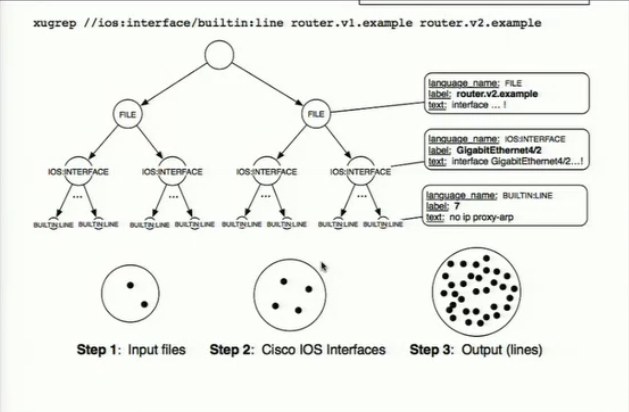
\includegraphics[scale=0.8]{xugrep}
          \caption{xugrep}
          \label{fig:xugrep}
        \end{figure}
\end{center}
\newpage

\subsection{xuwc}

Xuwc makes it possible to count text by understanding the structure for a specific language\footnote{IOS, C-language and XML}. So xuwc basically understands to language hierarchy in order to perform its job, which is counting \cite{xutools01}. \\

\underline{Use cases for xuwc:} \\ \\

\textbf{Network Configuration Management}: Perform easy and quick longitudinal studies on their own configuration data\\
\textbf{Developers}: Easily count the number of functions and lines per function\\
\textbf{Security Analysts}: Easily count the number of paragraphs per section or subsection of a policy and show the changes of by using the counting\\

\textcolor{red}{The concept is shown in figure~\ref{fig:xuwc}.}\\

\begin{center}
        \begin{figure}[h!]
          \centering
                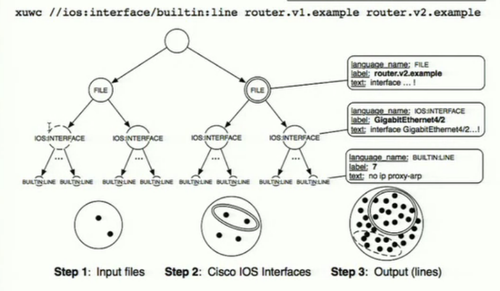
\includegraphics[scale=0.8]{xuwc}
          \caption{xuwc}
          \label{fig:xuwc}
        \end{figure}
\end{center}
\newpage

\subsection{xudiff}

Xudiff compares two files in terms of higher-level-language constructs \cite{xutools01}.\\

\underline{Use cases for xudiff:} \\ \\

\textbf{Network Configuration Management}: Capture the changes of configuration files to have a good overview of what changed\\
\textbf{Developers}: Capture the changes of a functions different levels\\
\textbf{Security Analyst}: Capture the changes of a section and subsection rather than per line\\

\textcolor{red}{The concept is shown in figure~\ref{fig:xudiff}.}\\

\begin{center}
        \begin{figure}[h!]
          \centering
                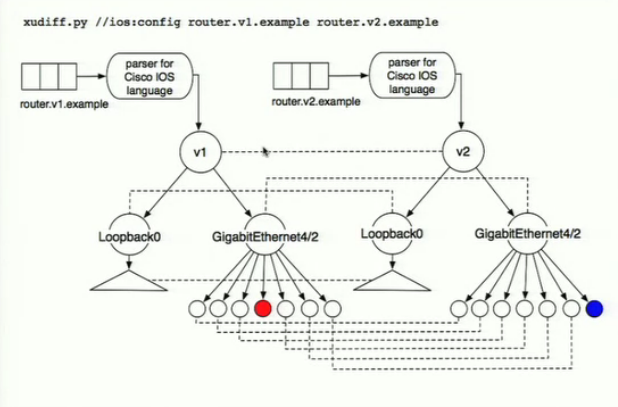
\includegraphics[scale=0.8]{xudiff}
          \caption{xudiff}
          \label{fig:xudiff}
        \end{figure}
\end{center}


% The bibliography
\begin{thebibliography}{9}

\bibitem{wk01}
   \textbf{Wikipedia},
   \emph{"AJAX"}.
<<<<<<< HEAD
   http://en.wikipedia.org/wiki/Ajax\_(programming)
   September 18, 2014 
\bibitem{jj05}
   \textbf{Jesse James Garrett},
   \emph{"Ajax: A New Approach to Web Applications"}.
   https://web.archive.org/web/20080702075113/http://www.adaptivepath.com/ideas/essays/archives/000385.php
   February 18, 2005
\bibitem{w3s}
   \textbf{w3schools},
   \emph{"AJAX Introduction"}.
   http://www.w3schools.com/ajax/ajax\_intro.asp
   February 18, 2005
=======
   \url{http://en.wikipedia.org/wiki/Ajax\_(programming)}
   18 September 2014 
\bibitem{jj05}
   \textbf{Jesse James Garrett},
   \emph{"Ajax: A New Approach to Web Applications"}.
   \url{https://web.archive.org/web/20080702075113/http://www.adaptivepath.com/ideas/essays/archives/000385.php}
   18 February 2005
\bibitem{w3s}
   \textbf{w3schools},
   \emph{"AJAX Introduction"}.
   \url{http://www.w3schools.com/ajax/ajax\_intro.asp}
   18 February 2005
>>>>>>> 4d6528585c683ed19f40f600bae7e80c2870553c
\bibitem{wk02}
   \textbf{Wikipedia},
   \emph{"JSON"}.
   http://en.wikipedia.org/wiki/JSON
<<<<<<< HEAD
   September 23, 2014
\bibitem{xutools01}
   \textbf{Gabriel A. Weaver and Sean W. Smith}
   \emph{"XUTools"}
   https://www.usenix.org/conference/lisa12/technical-sessions/presentation/weaver
   September 23, 2014
\end{thebibliography}
=======
   23 September 2014
\bibitem{XSL-FO}
  \textbf{Harvard cscie 153},
  \emph{"XSL-FO process"},
  \url{http://cscie153.dce.harvard.edu/lecture\_notes/2008/20081104/images/xslfo-process.png}
  24 September 2014
\bibitem{make_harmful}
  \textbf{Miller, P.A.} (1998), 
  \emph{"Recursive Make Considered Harmful"},
  AUUGN Journal of AUUG Inc., 19(1), pp. 14-25.
\end{thebibliography}
>>>>>>> 4d6528585c683ed19f40f600bae7e80c2870553c


\end{document}
